 \documentclass[12pt,dvipdfmx]{beamer}
\usepackage{pgfpages}
\usepackage{graphicx}
\DeclareGraphicsExtensions{.eps}
\usepackage{listings}
\usepackage{fancybox}
\usepackage{hyperref}

%%%%%%%%%%%%%%%%%%%%%%%%%%%
%%% themes
%%%%%%%%%%%%%%%%%%%%%%%%%%%
\usetheme{Szeged} 
%% no navigation bar
% default boxes Bergen Boadilla Madrid Pittsburgh Rochester
%% tree-like navigation bar
% Antibes JuanLesPins Montpellier
%% toc sidebar
% Berkeley PaloAlto Goettingen Marburg Hannover Berlin Ilmenau Dresden Darmstadt Frankfurt Singapore Szeged
%% Section and Subsection Tables
% Copenhagen Luebeck Malmoe Warsaw

%%%%%%%%%%%%%%%%%%%%%%%%%%%
%%% innerthemes
%%%%%%%%%%%%%%%%%%%%%%%%%%%
% \useinnertheme{circles}	% default circles rectangles rounded inmargin

%%%%%%%%%%%%%%%%%%%%%%%%%%%
%%% outerthemes
%%%%%%%%%%%%%%%%%%%%%%%%%%%
% outertheme
% \useoutertheme{default}	% default infolines miniframes smoothbars sidebar sprit shadow tree smoothtree


%%%%%%%%%%%%%%%%%%%%%%%%%%%
%%% colorthemes
%%%%%%%%%%%%%%%%%%%%%%%%%%%
\usecolortheme{seahorse}
%% special purpose
% default structure sidebartab 
%% complete 
% albatross beetle crane dove fly seagull 
%% inner
% lily orchid rose
%% outer
% whale seahorse dolphin

%%%%%%%%%%%%%%%%%%%%%%%%%%%
%%% fontthemes
%%%%%%%%%%%%%%%%%%%%%%%%%%%
\usefonttheme{serif}  
% default professionalfonts serif structurebold structureitalicserif structuresmallcapsserif

%%%%%%%%%%%%%%%%%%%%%%%%%%%
%%% generally useful beamer settings
%%%%%%%%%%%%%%%%%%%%%%%%%%%
% 
\AtBeginDvi{\special{pdf:tounicode EUC-UCS2}}
% do not show navigation
\setbeamertemplate{navigation symbols}{}
% show page numbers
\setbeamertemplate{footline}[frame number]


%%%%%%%%%%%%%%%%%%%%%%%%%%%
%%% define some colors for convenience
%%%%%%%%%%%%%%%%%%%%%%%%%%%

\newcommand{\mido}[1]{{\color{green}#1}}
\newcommand{\mura}[1]{{\color{purple}#1}}
\newcommand{\ore}[1]{{\color{orange}#1}}
\newcommand{\ao}[1]{{\color{blue}#1}}
\newcommand{\aka}[1]{{\color{red}#1}}

\setbeamercolor{ex}{bg=cyan!20!white}

%%%%%%%%%%%%%%%%%%%%%%%%%%%
%%% how to typset code
%%%%%%%%%%%%%%%%%%%%%%%%%%%

\lstset{language = C,
numbers = left,
numberstyle = {\tiny \emph},
numbersep = 10pt,
breaklines = true,
breakindent = 40pt,
frame = tlRB,
frameround = ffft,
framesep = 3pt,
rulesep = 1pt,
rulecolor = {\color{blue}},
rulesepcolor = {\color{blue}},
flexiblecolumns = true,
keepspaces = true,
basicstyle = \ttfamily\scriptsize,
identifierstyle = ,
commentstyle = ,
stringstyle = ,
showstringspaces = false,
tabsize = 4,
escapechar=\@,
}

\title{数学・物理をプログラミングで考える}
\institute{}
\author{田浦健次朗・山崎俊彦}
\date{}

\AtBeginSubsection[] % Do nothing for \section*
{
\begin{frame}
\frametitle{Contents}
\tableofcontents[currentsection,currentsubsection]
\end{frame}
}

\begin{document}
\maketitle

%%%%%%%%%%%%%%%%% 
\begin{frame}
\frametitle{モットー}
\begin{itemize}
\item プログラミングを生き生きと学ぶ
  \begin{itemize}
  \item 実際の問題解決(数学や物理)に適用する
  \end{itemize}
\item 数学や物理を生き生きと学ぶ
  \begin{itemize}
  \item 多次元の線形代数,多変数の微分(ベクトル解析),
    多次元の積分,微分方程式,偏微分方程式,\ldots
  \item コンピュータによる数値計算は「実用的・本当の使い道」のひとつ
  \end{itemize}
\end{itemize}

\[
\left(
\begin{array}{ccc}
a_{11}    & \cdots & a_{1n}    \\
\vdots   & \ddots & \vdots \\
a_{m1}    & \cdots & a_{mn}    \\
\end{array}
\right), 
\nabla^2 \phi = \rho, 
\int_C f(x) \cdot d\vec{s}, 
\ldots
\]
\end{frame}

%%%%%%%%%%%%%%%%% 
\begin{frame}
\frametitle{進め方}
\begin{itemize}
\item 「問題(候補)」をいくつか示す
  \begin{itemize}
  \item 入門から徐々に高度・一般的なものも
  \end{itemize}
\item プログラミングなど,道具に関する最低限の講義と演習
\item 数人のグループを作る
\item グループによる,問題解決に向けた議論,作業(プログラミング)
\item 途中経過の発表,全体議論
\item 最終発表
\end{itemize}
\end{frame}

%%%%%%%%%%%%%%%%% 
\begin{frame}
\frametitle{問題例}
\begin{itemize}
\item 見覚えがある :-)

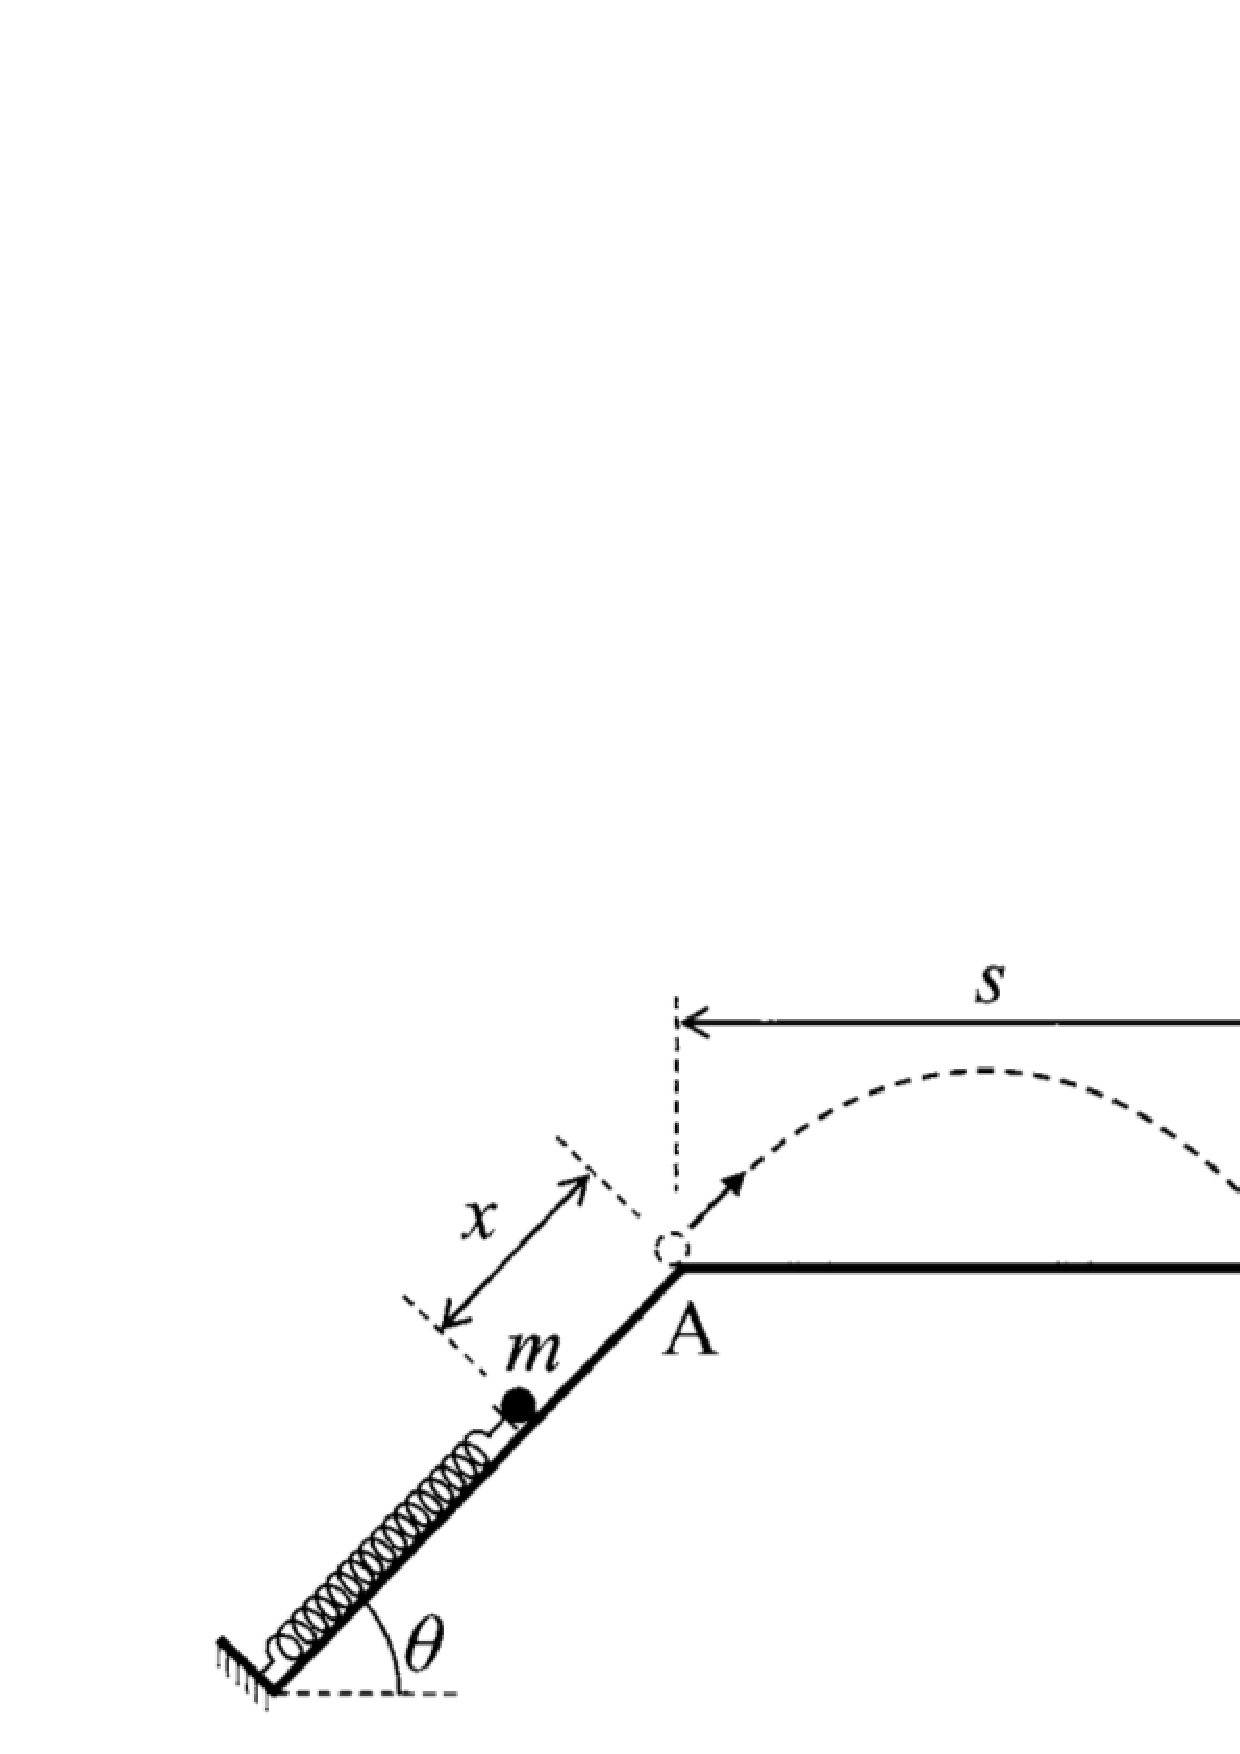
\includegraphics[width=\textwidth]{out/pdf/img/physics.pdf}

\item $\theta$がいくつのときに,最も遠くまで飛ぶか?
\end{itemize}
\end{frame}

%%%%%%%%%%%%%%%%% 
\begin{frame}
\frametitle{「問題」の例}
\begin{itemize}
\item ゲームの最適な戦略を考える
\end{itemize}

\begin{center}
\begin{tabular}{ll}

\includegraphics[height=0.3\textwidth]{out/pdf/img/algo-cards.pdf}
&    
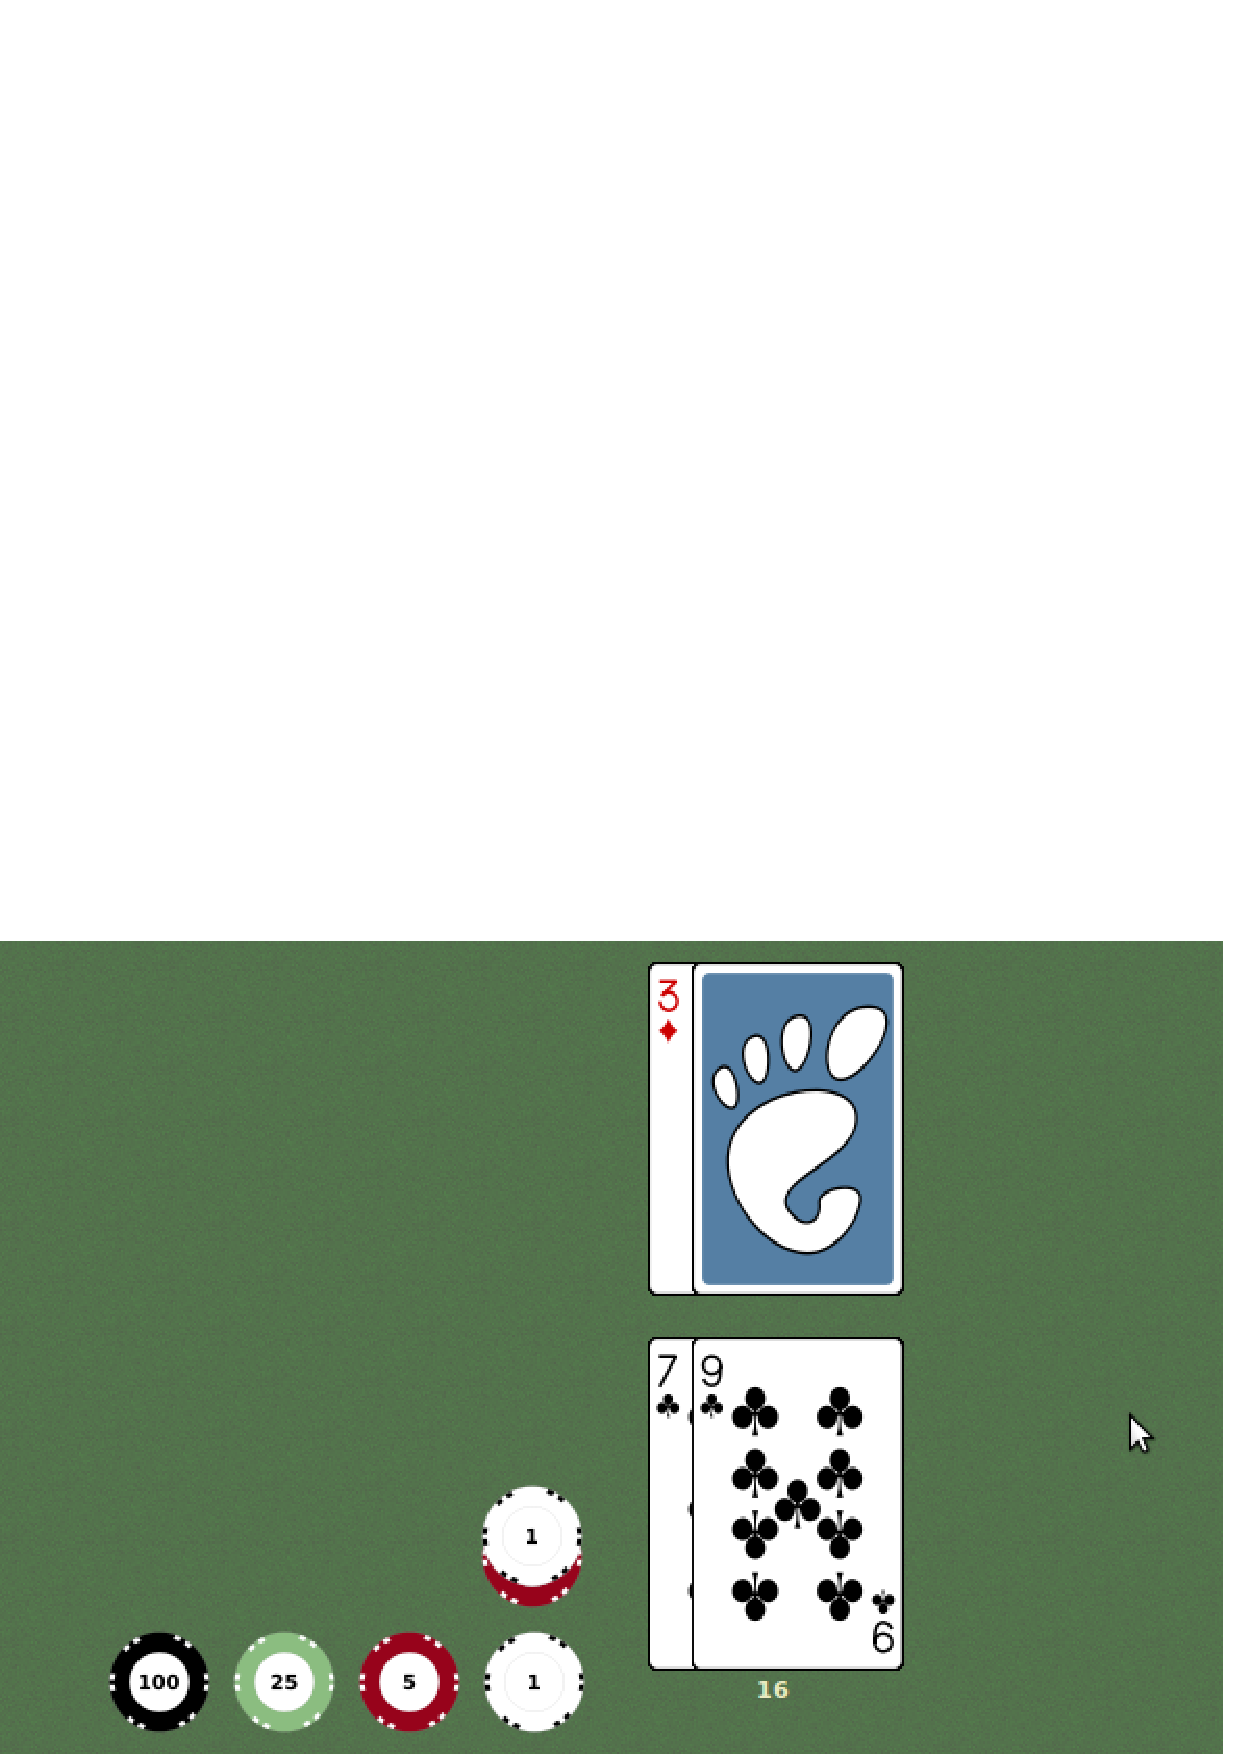
\includegraphics[height=0.3\textwidth]{out/pdf/img/blackjack.pdf}
\\
{\scriptsize http://www.sansu-olympic.gr.jp/algo/}
\end{tabular}
\end{center}
\end{frame}

%%%%%%%%%%%%%%%%% 
\begin{frame}
\frametitle{問題の背景}
\begin{tabular}{|c|c|}\hline
確率 & 乱数を用いたシミュレーション \\
積分 & 数値的な積分,乱数の利用 \\
関数の最大最小 & 力づく,勾配を利用した最小・最大の探索 \\
微分方程式 & 数値的な積分 \\
シミュレーション & 数値的な積分 \\\hline
\end{tabular}
\end{frame}


%%%%%%%%%%%%%%%%% 
\begin{frame}
\frametitle{ゼミの目標}
\begin{itemize}
\item プログラミングはマスターする価値のある道具
\item コンピュータによる計算原理の単純さ,強力さ
\item やってる計算そのものが単純でも,
正しいことの吟味,効率的な計算の発明には数学が必要
\begin{itemize}
\item 100次元の積分,100変数の最大・最小は力づくでは無理
\item この計算の誤差はどのくらい?
\item このシミュレーション結果何か変\ldots
\end{itemize}

\item 
\[
\left(
\begin{array}{ccc}
a_{11}    & \cdots & a_{1n}    \\
\vdots   & \ddots & \vdots \\
a_{m1}    & \cdots & a_{mn}    \\
\end{array}
\right), 
\nabla^2 \phi = \rho, 
\int_C f(x) \cdot d\vec{s}, 
\ldots
\]
などが,生き生きと,有用な道具と感じられるように\ldots
\end{itemize}
\end{frame}

\end{document}



